\documentclass[conference]{IEEEtran}
\IEEEoverridecommandlockouts

\usepackage{cite}
\usepackage{amsmath,amssymb,amsfonts}
\usepackage{algorithmic}
\usepackage{graphicx}
\usepackage{textcomp}
\usepackage{xcolor}
\def\BibTeX{{\rm B\kern-.05em{\sc i\kern-.025em b}\kern-.08em
    T\kern-.1667em\lower.7ex\hbox{E}\kern-.125emX}}

\renewcommand{\figurename}{Gambar}
\renewcommand{\tablename}{Tabel}
\renewcommand{\IEEEkeywordsname}{Keywords}
\usepackage{caption}
\usepackage{pgf}

\begin{document}
    
\title{Intrusion Detection}

\author{\IEEEauthorblockN{Erwin Erikson}
\IEEEauthorblockA{\textit{Faculty of Information Technology} \\
\textit{Institut Teknologi Batam}\\
Batam, Indonesia \\
1822003@student.iteba.ac.id}
\and
\IEEEauthorblockN{Muhammad Al Imron}
\IEEEauthorblockA{\textit{Faculty of Information Technology} \\
\textit{Institut Teknologi Batam}\\
Batam, Indonesia \\
1822007@student.iteba.ac.id}
\and
\IEEEauthorblockN{Farhan Ghulam Hadi Saputra}
\IEEEauthorblockA{\textit{Faculty of Information Technology} \\
\textit{Institut Teknologi Batam}\\
Batam, Indonesia \\
1822014@student.iteba.ac.id}
}

\maketitle

\begin{abstract}
Meningkatnya perkembangan internet tidak terlepas dari serangan seperti malware infection. Intrusion Detection System (IDS) adalah masalah nonlinier, rumit dan berhubungan dengan data lalu lintas jaringan. IDS mencoba untuk mengidentifikasi dan memberi tahu aktivitas pengguna sebagai anomali normal. Untuk mendeteksi berbagai serangan jaringan dapat dilatih dengan melakukan percobaan menggunakan dataset NSL-KDD dengan beberapa algoritma yaitu Random Forest, K-Neighbors, SVM dan Ensemble Learning.
\end{abstract}

\begin{IEEEkeywords}
intrusion detection, Random Forest, K-Neighbors, SVM, Ensemble Learning, NSL-KDD dataset.
\end{IEEEkeywords}

\section{Pendahuluan}
Pengguna internet yang terus meningkat dari tahun ke tahun tidak terlepas dari serangan yang timbul dari teknologi jaringan seperti serangan \emph{malware infection}. Oleh karena itu, diperlukan keamanan dalam sistem komputer untuk mencegah dari serangan.

IDS (\emph{Intrusion Detection System}) merupakan sebuah aplikasi yang mampu mencatat kegiatan dalam suatu jaringan dan menganalisa paket-paket yang dikirim melalui lalu lintas jaringan secara \emph{realtime}. Tujuan dari sistem ini yaitu mengawasi jika terjadi penetrasi ke dalam sistem, mengawasi \emph{traffic} yang terjadi pada jaringan, mendeteksi \emph{anomaly} terjadinya penyimpangan dari sistem yang normal atau tingkah laku user.

Dalam melakukan deteksi serangan, dapat digunakan beberapa algoritma  yaitu Random Forest, K-Neighbors, SVM dan Ensemble Learning. Dan tujuan dari penelitian ini adalah untuk membandingkan performa dari masing-masing algoritma.

\section{Penjelasan Teori}

\subsection{Random Forest}

Hutan acak (\emph{Random Forest}) adalah kumpulan pohon keputusan yang digunakan untuk meningkatkan akurasi, biasanya dilatih dengan metode "\emph{bagging}". Ide umum dari metode \emph{bagging} adalah bahwa kombinasi model pembelajaran meningkatkan hasil secara keseluruhan.

Keuntungan \emph{Random Forest} adalah sebagai berikut\cite{farnaaz2016random}:

\begin{enumerate}
\item Hutan yang dihasilkan dapat disimpan untuk referensi di masa mendatang.
\item Hutan acak mengatasi masalah penyesuaian.
\item Dalam akurasi RF dan kepentingan variabel secara otomatis dihasilkan.
\end{enumerate}

Flowchart dari proses pemodelan algoritma \emph{Random Forest} dapat dilihat pada ``Gambar. 1''.\vspace{6pt}

\begin{minipage}{\linewidth}
\centerline{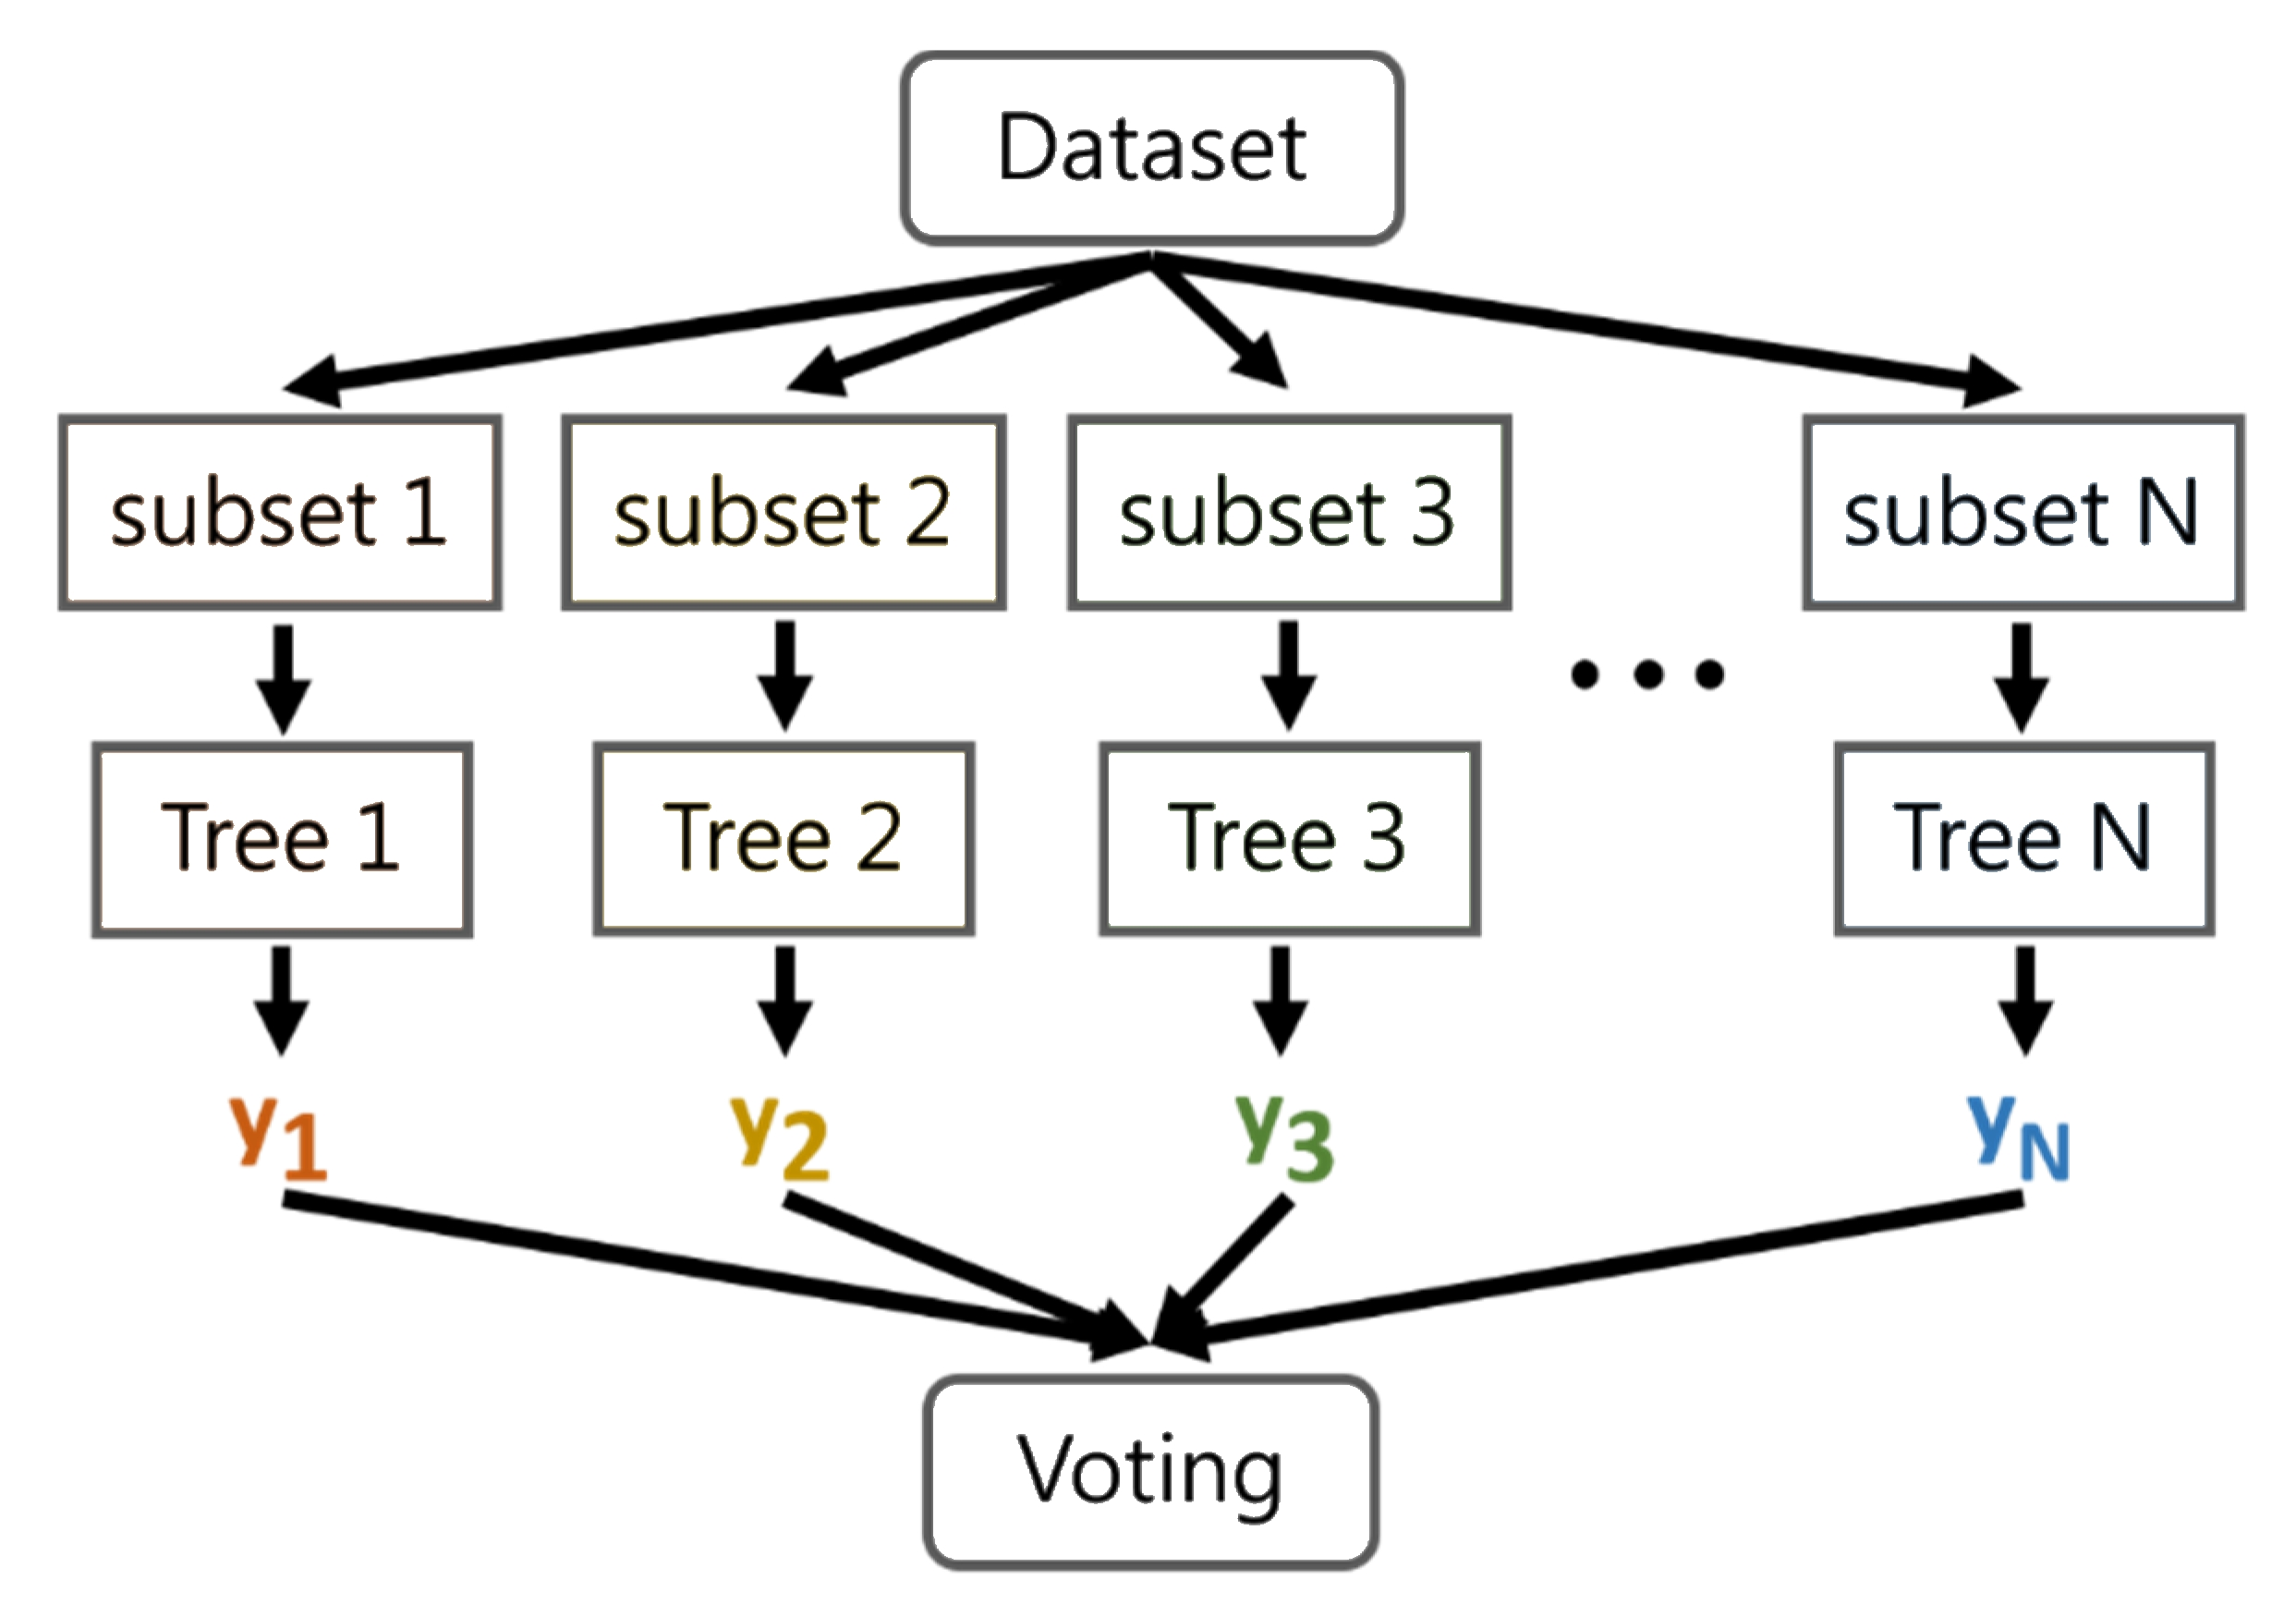
\includegraphics[width=60mm]{Gambar/Gbr001.jpg}}
\captionof{figure}{Flowchart Algoritma Random Forest}
\label{fig1}
\end{minipage}

\subsection{K-Nearest Neighbors}

\emph{K-nearest neighbors} (knn) adalah algoritma yang berfungsi untuk melakukan klasifikasi suatu data berdasarkan data pembelajaran (\emph{train data sets}), yang diambil dari k tetangga terdekatnya (\emph{nearest neighbors}), dengan k merupakan banyaknya tetangga terdekat\cite{liao}. Beberapa formula yang digunakan adalah:

\begin{itemize}
\item \emph{Euclidean Distance}\\
Untuk mendefinisikan jarak antara dua titik yaitu titik pada data training (x) dan titik pada data testing (y), maka digunakan rumus \emph{Euclidean}\cite{nurhadi2017aplikasi}, yaitu:

\begin{equation*}
d(x,y)=\sqrt{\sum^{n}_{i=1} (x_i-y_i)^2}
\label{eq1}
\end{equation*}

dimana:

$d$ = jarak antara 2 titik

$x$ = data uji

$y$ = data latih

$i$ = merepresentasikan nilai atribut

$n$ = merupakan dimensi atribut.\vspace{10pt}

\item \emph{City Block Distance}\\
\emph{City Block Distance} umumnya dihitung antara 2 koordinat objek yang berpasangan. Ini adalah penjumlahan dari perbedaan absolut antara 2 koordinat. \emph{City Block Distance} 2-titik a dan b dengan dimensi k dihitung secara matematis menggunakan rumus berikut ini:

\begin{equation*}
d_{ij}=\sum^{k}_{i=1} | a_i-b_i |
\label{eq2}
\end{equation*}

\item \emph{Manhattan Distance}\\
\emph{Manhattan Distance} merupakan salah satu pengukuran yang paling banyak digunakan meliputi penggantian perbedaan kuadrat dengan menjumlahkan perbedaan \emph{absolute} dari variabel-variabel. Fungsi ini hanya akan menjumlahkan selisih nilai x dan y dari dua buah titik.
\vspace{10pt}

\item \emph{Minkwoski Distance}\\
\emph{Minkwoski Distance} adalah metrik dalam ruang vektor bernorma yang dapat dianggap sebagai generalisasi dari kedua jarak \emph{Euclidean} dan jarak \emph{Manhattan}. Jarak \emph{Minkowski} antara dua variabel X dan Y didefinisikan sebagai:

\begin{equation*}
d = (\sum^{n}_{i=1} | X_i-Y_i |^p)^{1/p}
\label{eq3}
\end{equation*}

Kasus di mana $p$ = 1 setara dengan jarak \emph{Manhattan} dan kasus di mana $p$ = 2 setara dengan jarak \emph{Euclidean}.

\end{itemize}

Flowchart dari proses pemodelan algoritma \emph{K-nearest neighbors} dapat dilihat pada ``Gambar. 2''\cite{lubis2020optimization}.\vspace{6pt}

\begin{minipage}{\linewidth}
\centerline{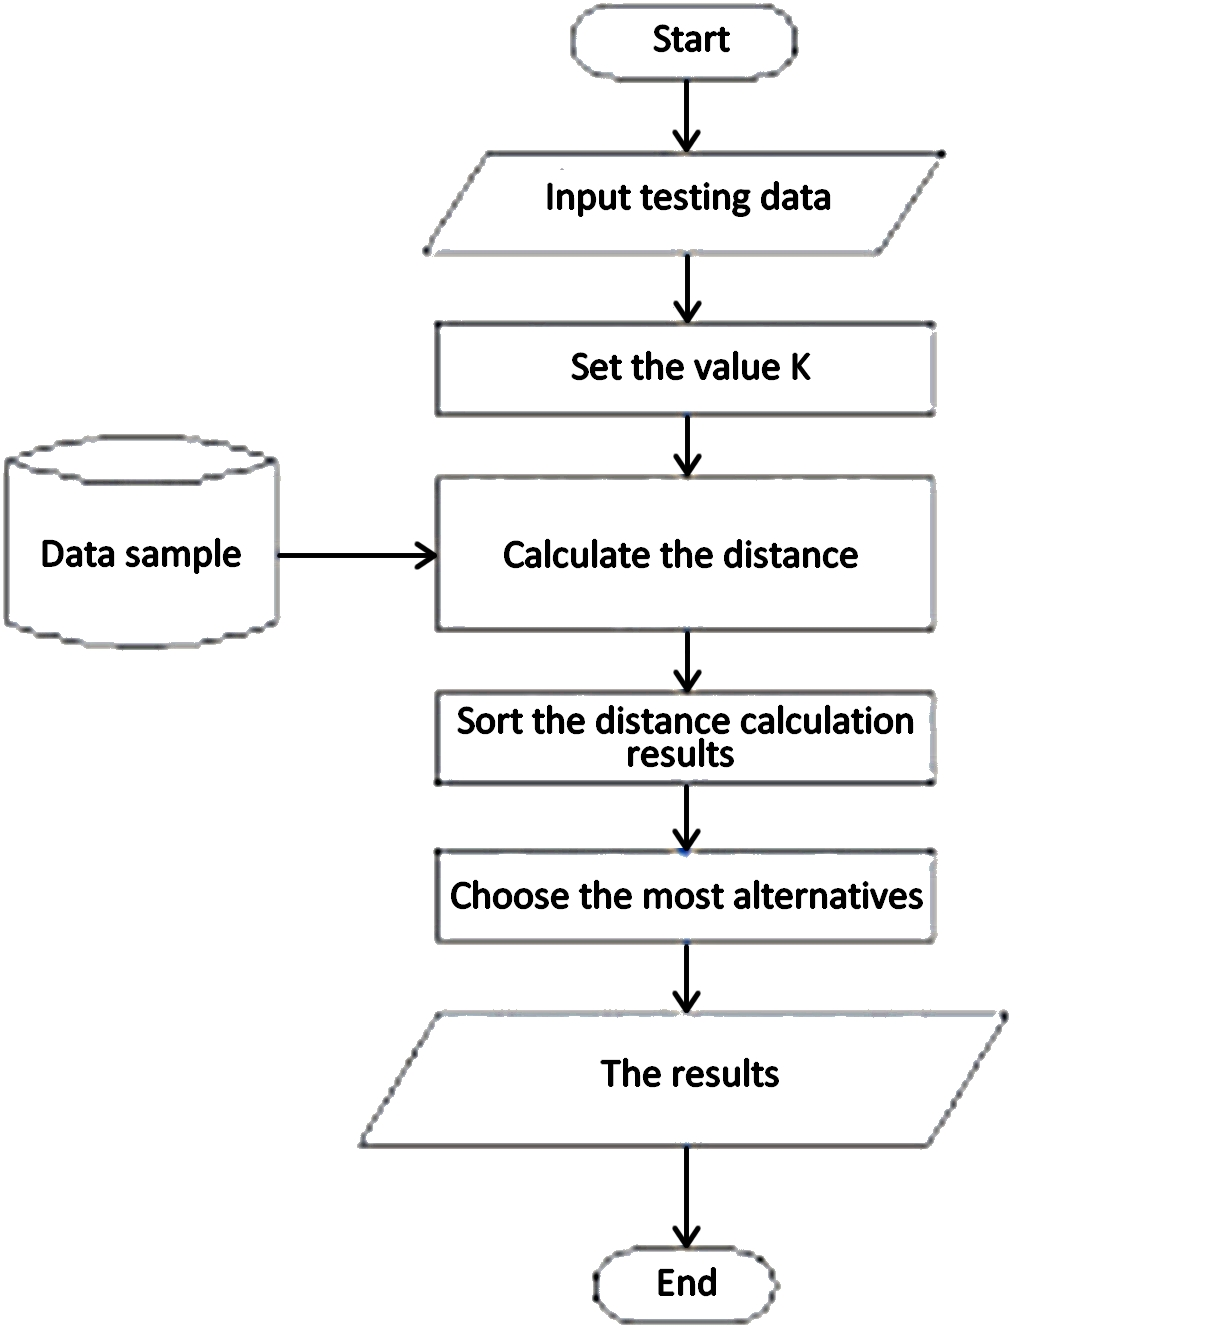
\includegraphics[width=55mm]{Gambar/Gbr002.jpg}}
\captionof{figure}{Flowchart Algoritma K-nearest neighbors}
\label{fig2}
\end{minipage}

\subsection{SVM}

Teori SVM berasal dari statistik dan prinsip dasar SVM adalah menemukan \emph{hyperplane} linier yang optimal dalam ruang fitur yang secara maksimal memisahkan dua kelas target\cite{hasan}.

Dalam kaitannya dengan fungsi kernel, fungsi diskriminan mengambil bentuk berikut:

\begin{equation*}
f(x) = \sum^{n}_i \alpha_ik(x,x_i)+b
\label{eq4}
\end{equation*}

Dalam pekerjaan ini, kernel \emph{Gaussian} telah digunakan
untuk membangun pengklasifikasi SVM.\\ \emph{Gaussian} kernel:

\begin{equation*}
K(x_i,x_j) = exp\left (- \frac{||x_i-x_j||^2}{2\sigma} \right )
\label{eq5}
\end{equation*}

\noindent dimana $\sigma$ adalah lebar fungsi.

Fungsi kernel dan parameternya harus dipilih untuk membangun pengklasifikasi SVM. Melatih SVM menemukan \emph{hyperplane} margin besar, yaitu menetapkan parameter $\alpha$.

Flowchart dari proses pemodelan algoritma SVM dapat dilihat pada ``Gambar. 3''\cite{inproceedings}.\vspace{6pt}

\begin{minipage}{\linewidth}
\centerline{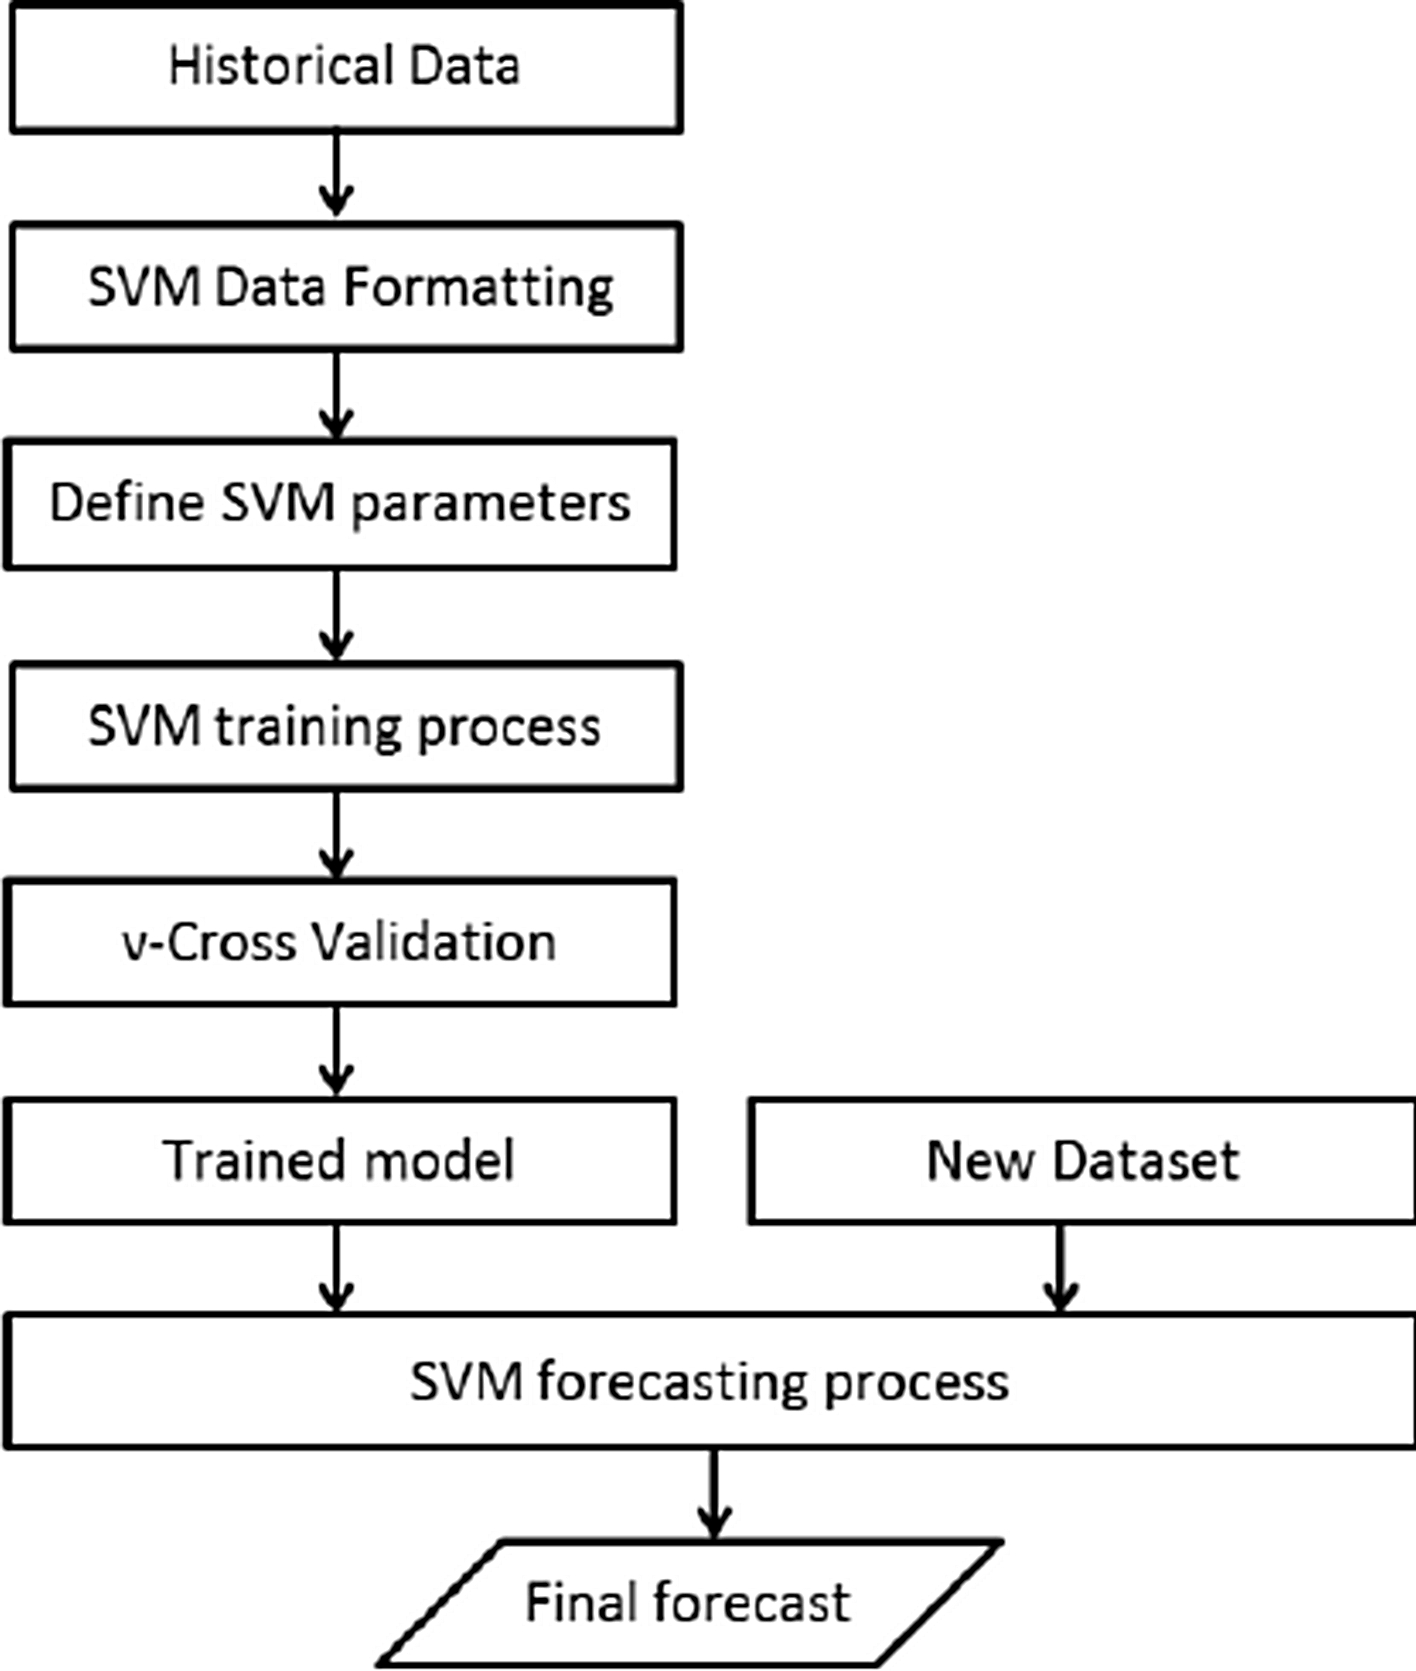
\includegraphics[width=50mm]{Gambar/Gbr003.jpg}}
\captionof{figure}{Flowchart Algoritma SVM}
\label{fig3}
\end{minipage}

\subsection{Ensemble Learning}

Metode ini adalah menggabungkan beberapa fitur dengan pembelajaran \emph{Ensemble}.

Flowchart dari proses pemodelan algoritma \emph{Ensemble Learning} dapat dilihat pada ``Gambar. 4''\cite{zhang}.\vspace{6pt}

\begin{minipage}{\linewidth}
\centerline{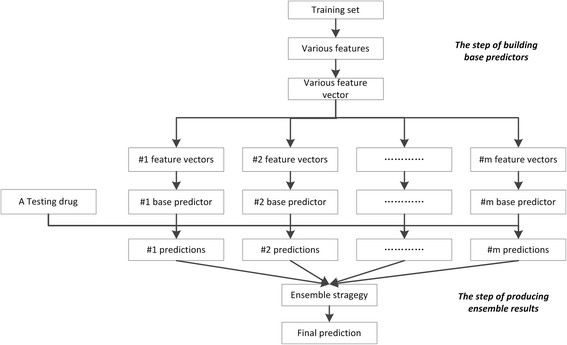
\includegraphics[width=80mm]{Gambar/Gbr004.png}}
\captionof{figure}{Flowchart Algoritma Ensemble Learning}
\label{fig4}
\end{minipage}

\section{Metodologi}

Metodologi adalah tahapan yang akan dilakukan dalam melakukan penelitian agar dapat memenuhi tujuan sesuai dengan yang diharapkan. Tahapan penelitian yang akan dilakukan dapat dilihat pada ``Gambar. 5''.

\begin{minipage}{\linewidth}
\centerline{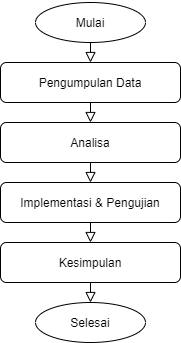
\includegraphics[width=35mm]{Gambar/Metodologi_Diagram.png}}
\captionof{figure}{Tahapan Penelitian}
\label{fig5}
\end{minipage}
\vspace{6pt}

Tahapan pada penelitian ini dapat dijelaskan sebagai berikut:

\noindent \textbf{Pengumpulan Data}

Pengumpulan data yang dilakukan dengan membaca dan mempelajari penelitian sebelumnya yang berhubungan dengan IDS.

\noindent \textbf{Analisa}

Pada tahap ini adalah menganalisa data yaitu data latih yang digunakan untuk standarisasi melakukan pengujian, dan data uji yang digunakan untuk mengetes penilaian yang dihasilkan
dari data latih.

Tahap ini juga menganalisa metode yang digunakan dalam penelitian yang berkaitan dengan sistem yang digunakan.

\noindent \textbf{Implementasi dan Pengujian}

Proses implementasi adalah merealisasikan aplikasi IDS sesuai dengan dengan bahasa pemrograman yang digunakan yaitu Phyton menggunakan JupyterLab.

Tahap pengujian adalah tahap yang dilakukan untuk menguji masing-masing metode yang digunakan dalam penelitian dengan tujuan untuk mengetahui perbandingan performa dari setiap algoritma.

\noindent \textbf{Kesimpulan}

Merupakan tahap penentuan kesimpulan terhadap hasil pengujian yang telah dilakukan.

\section{Hasil dan Pembahasan}

Untuk melakukan pelatihan/pengujian digunakan dataset NSL-KDD dimana NSL\_KDD\_Train sebagai data latih dan NSL\_KDD\_Test sebagai data uji seperti pada ``Gambar. 6''\cite{mamcose}.\vspace{6pt}

\begin{minipage}{\linewidth}
\centerline{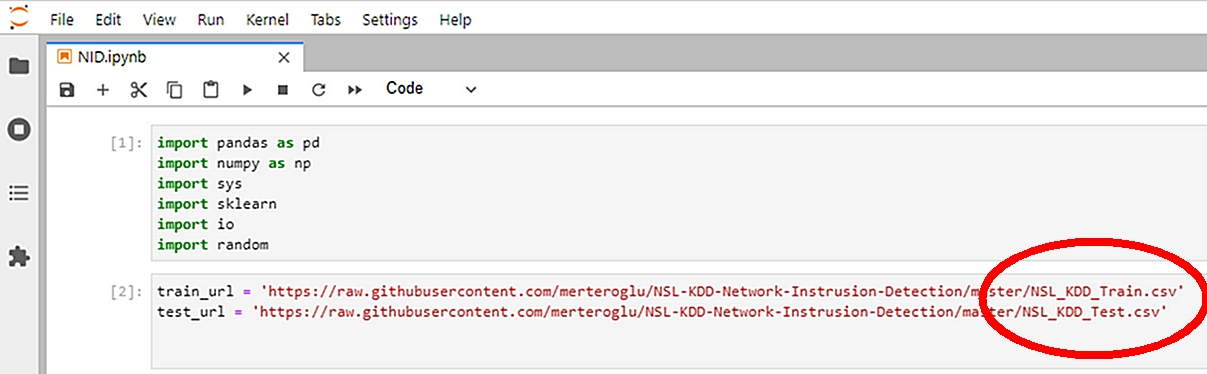
\includegraphics[width=80mm]{Gambar/Gbr01.jpg}}
\captionof{figure}{Data Latih dan Data Uji}
\label{fig6}
\end{minipage}
\vspace{6pt}

Dari dataset tersebut dibagi untuk setiap kategori serangan
yaitu 0 = Normal, 1 = DoS, 2 = Probe, 3 = R2L, 4 = U2R.
Hasil pembagian setiap kategori serangan dari data latih dan data uji dapat dilihat pada ``Gambar. 7''.\vspace{6pt}

\begin{minipage}{\linewidth}
    \centerline{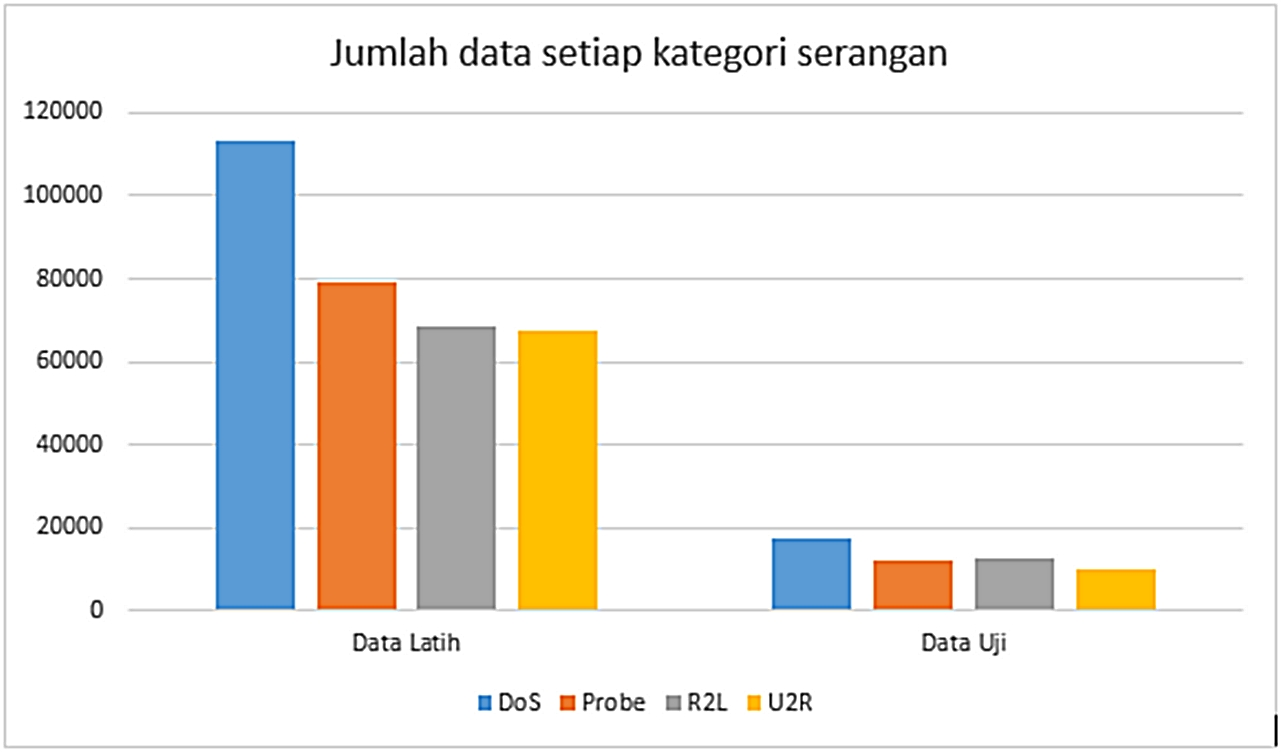
\includegraphics[width=80mm]{Gambar/Gbr011.jpg}}
    \captionof{figure}{Jumlah Data Setiap Kategori Serangan}
    \label{fig7}
    \end{minipage}
    \vspace{6pt}

Untuk menghitung precision dan recall dengan cepat dari setiap serangan dilakukan
tahap \emph{Prediction} dan \emph{Evaluation} (\emph{validation}) dengan \emph{confusion matrix}
seperti pada ``Gambar. 8''.

\begin{minipage}{\linewidth}
\centerline{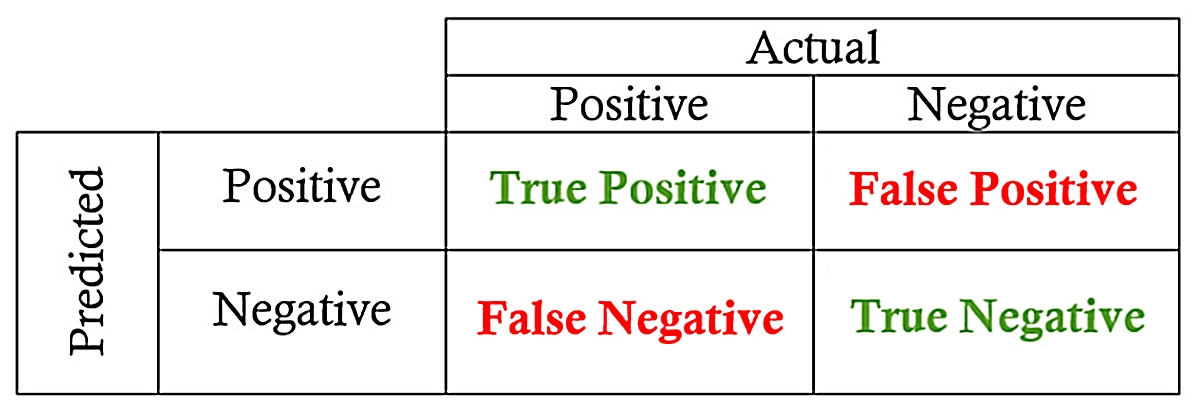
\includegraphics[width=60mm]{Gambar/Gbr005.jpg}}
\captionof{figure}{Confusion Matrix}
\label{fig8}
\end{minipage}
\vspace{6pt}


Hasil \emph{Prediction} dan \emph{Evaluation} (\emph{validation})
metode \emph{Random Forest} semua fitur dapat dilihat
pada ``Gambar. 9''.

\begin{minipage}{\linewidth}
\centerline{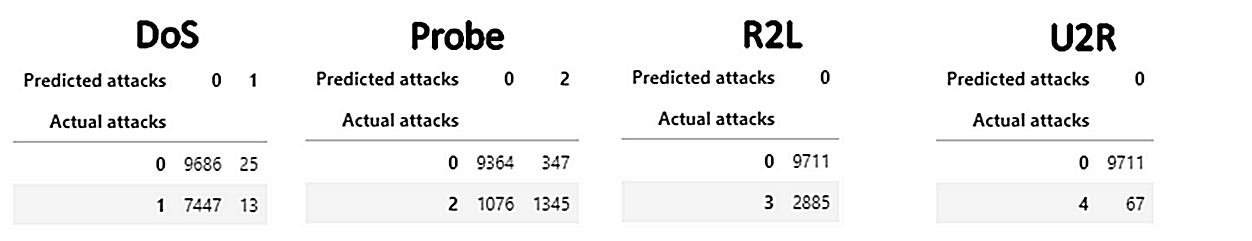
\includegraphics[width=90mm]{Gambar/Gbr006.jpg}}
\captionof{figure}{Confusion Matrix Random Forest All Fitur}
\label{fig9}
\end{minipage}
\vspace{6pt}

Hasil \emph{Prediction} dan \emph{Evaluation} (\emph{validation})
metode \emph{Random Forest} 13 fitur dapat dilihat
pada ``Gambar. 10''.

\begin{minipage}{\linewidth}
\centerline{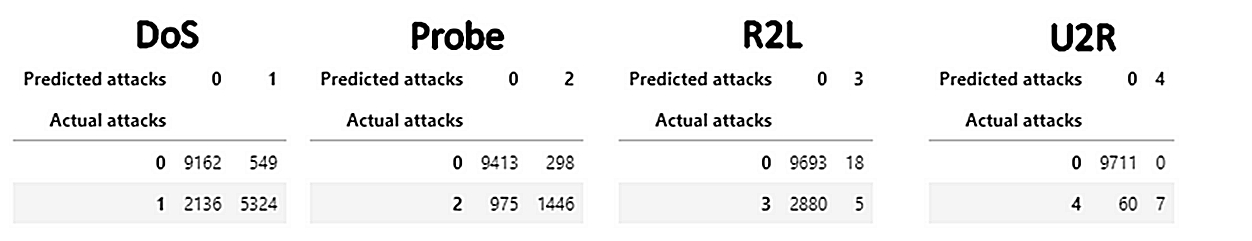
\includegraphics[width=90mm]{Gambar/Gbr007.jpg}}
\captionof{figure}{Confusion Matrix Random Forest 13 Fitur}
\label{fig10}
\end{minipage}
\vspace{6pt}

Hasil \emph{Prediction} dan \emph{Evaluation} (\emph{validation})
metode \emph{K-Neighbors} dapat dilihat
pada ``Gambar. 11''.

\begin{minipage}{\linewidth}
\centerline{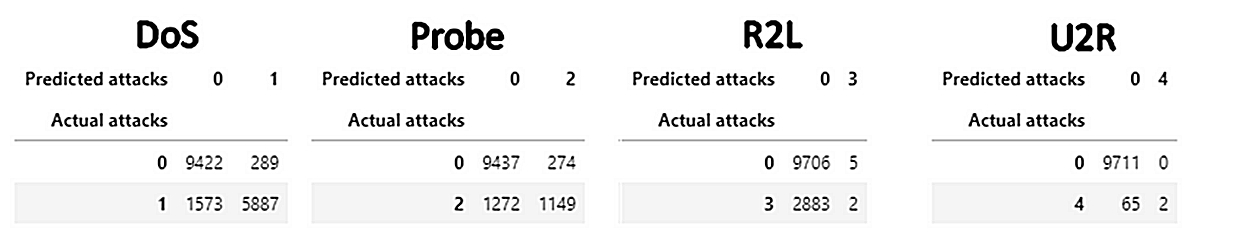
\includegraphics[width=90mm]{Gambar/Gbr008.jpg}}
\captionof{figure}{Confusion Matrix K-Neighbors}
\label{fig11}
\end{minipage}
\vspace{6pt}

Hasil \emph{Prediction} dan \emph{Evaluation} (\emph{validation})
metode SVM dapat dilihat
pada ``Gambar. 12''.

\begin{minipage}{\linewidth}
\centerline{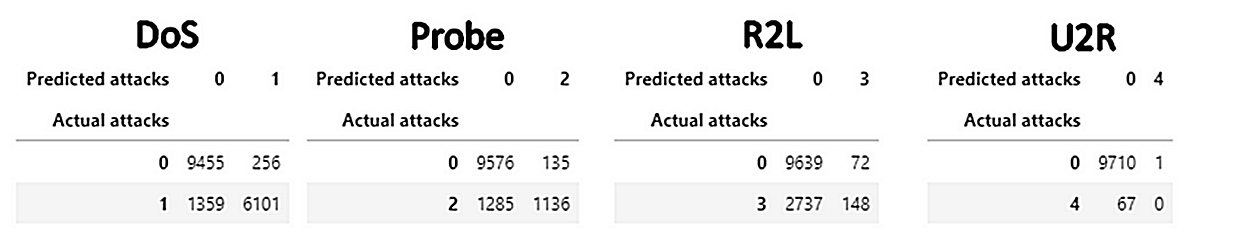
\includegraphics[width=90mm]{Gambar/Gbr009.jpg}}
\captionof{figure}{Confusion Matrix SVM}
\label{fig12}
\end{minipage}
\vspace{6pt}

Hasil \emph{Prediction} dan \emph{Evaluation} (\emph{validation})
metode \emph{Ensemble Learning} dapat dilihat
pada ``Gambar. 13''.

\begin{minipage}{\linewidth}
\centerline{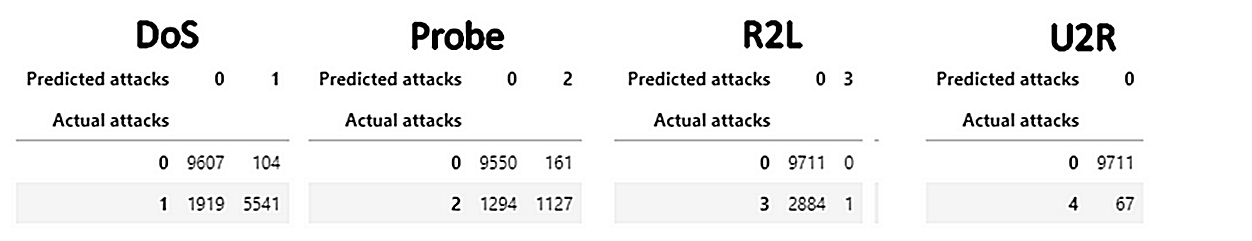
\includegraphics[width=90mm]{Gambar/Gbr010.jpg}}
\captionof{figure}{Confusion Matrix Ensemble Learning}
\label{fig13}
\end{minipage}
\vspace{6pt}

Dengan \emph{confusion matrix} dilakukan penghitungan \emph{Accuracy}, \emph{Precision}, \emph{Recall},
dan \emph{F-measure} dari nilai masing-masing dalam matriks dengan menerapkan persamaan berikut:

\begin{equation*}
    Accuracy = \frac{TP + TN}{TP + FP + FN + TN}
    \label{eq6}
\end{equation*}

\begin{equation*}
    Precision = \frac{TP}{TP + FP}
    \label{eq7}
\end{equation*}

\begin{equation*}
    Recall = \frac{TP}{TP + FN}
    \label{eq8}
\end{equation*}

\begin{equation*}
    F-measure = 2 * \frac{precision * recall}{precision + recall}
    \label{eq9}
\end{equation*}

\noindent dimana:

\noindent $TP$ = True Positive

\noindent $TN$ = True Negative

\noindent $FP$ = False Positive

\noindent $FN$ = False Negative
\vspace{6pt}

Dari hasil evaluasi kinerja dari masing-masing model atau algoritma, dapat dilihat pada tabel-tabel berikut:

\noindent Pengujian menggunakan algoritma \emph{Random Forest} untuk semua fitur dapat dilihat pada ``Tabel. I''.\vspace{6pt}

\begin{minipage}{\linewidth}
\captionof{table}{Algoritma Random Forest untuk semua Fitur}
\begin{center}
\begin{tabular}{|l|l|l|l|l|}
\hline
\multicolumn{1}{|c|}{\textbf{}}&\multicolumn{1}{|c|}{\textbf{Accuracy}}&\multicolumn{1}{|c|}{\textbf{Precision}}&\multicolumn{1}{|c|}{\textbf{Recall}}&\multicolumn{1}{|c|}{\textbf{F-measure}} \\
\hline
DoS & 0.99796 & 0.99906 & 0.99651 & 0.99765\\
\hline
Probe & 0.99670 & 0.99675 & 0.99262 & 0.99469\\
\hline
R2L & 0.99775 & 0.94964 & 0.82014 & 0.87775\\
\hline
U2R & 0.98047 & 0.97293 & 0.96844 & 0.97290\\
\hline
\end{tabular}
\label{tab1}
\end{center}
\end{minipage}\\ \\

\noindent Pengujian menggunakan algoritma \emph{Random Forest} untuk 13 fitur dapat dilihat pada ``Tabel. II''.\vspace{6pt}

\begin{minipage}{\linewidth}
\captionof{table}{Algoritma Random Forest untuk 13 Fitur}
\begin{center}
\begin{tabular}{|l|l|l|l|l|}
\hline
\multicolumn{1}{|c|}{\textbf{}}&\multicolumn{1}{|c|}{\textbf{Accuracy}}&\multicolumn{1}{|c|}{\textbf{Precision}}&\multicolumn{1}{|c|}{\textbf{Recall}}&\multicolumn{1}{|c|}{\textbf{F-measure}} \\
\hline
DoS & 0.99796 & 0.99839 & 0.99651 & 0.99718\\
\hline
Probe & 0.99382 & 0.98973 & 0.98668 & 0.98758\\
\hline
R2L & 0.97856 & 0.97280 & 0.96525 & 0.96838\\
\hline
U2R & 0.99693 & 0.96256 & 0.83183 & 0.90644\\
\hline
\end{tabular}
\label{tab2}
\end{center}
\end{minipage}\\ \\

\noindent Pengujian menggunakan algoritma \emph{K-Neighbors} dapat dilihat pada ``Tabel. III''.\vspace{6pt}

\begin{minipage}{\linewidth}
\captionof{table}{Algoritma K-Neighbors}
\begin{center}
\begin{tabular}{|l|l|l|l|l|}
\hline
\multicolumn{1}{|c|}{\textbf{}}&\multicolumn{1}{|c|}{\textbf{Accuracy}}&\multicolumn{1}{|c|}{\textbf{Precision}}&\multicolumn{1}{|c|}{\textbf{Recall}}&\multicolumn{1}{|c|}{\textbf{F-measure}} \\
\hline
DoS & 0.99715 & 0.99678 & 0.99665 & 0.99672\\
\hline
Probe & 0.99077 & 0.98606 & 0.98508 & 0.98553\\
\hline
R2L & 0.96705 & 0.95265 & 0.95439 & 0.95344\\
\hline
U2R & 0.99703 & 0.93143 & 0.85073 & 0.87831\\
\hline
\end{tabular}
\label{tab3}
\end{center}
\end{minipage}\\ \\

\noindent Pengujian menggunakan algoritma SVM dapat dilihat pada ``Tabel. IV''.

\begin{minipage}{\linewidth}
\captionof{table}{Algoritma SVM}
\begin{center}
\begin{tabular}{|l|l|l|l|l|}
\hline
\multicolumn{1}{|c|}{\textbf{}}&\multicolumn{1}{|c|}{\textbf{Accuracy}}&\multicolumn{1}{|c|}{\textbf{Precision}}&\multicolumn{1}{|c|}{\textbf{Recall}}&\multicolumn{1}{|c|}{\textbf{F-measure}} \\
\hline
DoS & 0.99371 & 0.99107 & 0.99450 & 0.99278\\
\hline
Probe & 0.98450 & 0.96907 & 0.98365 & 0.97613\\
\hline
R2L & 0.96793 & 0.94854 & 0.96264 & 0.95529\\
\hline
U2R & 0.99632 & 0.91056 & 0.82909 & 0.84869\\
\hline
\end{tabular}
\label{tab4}
\end{center}
\end{minipage}\\ \\

\noindent Pengujian menggunakan algoritma \emph{Ensemble Learning} dapat dilihat pada ``Tabel. V''.\vspace{6pt}

\begin{minipage}{\linewidth}
\captionof{table}{Algoritma Ensemble Learning}
\begin{center}
\begin{tabular}{|l|l|l|l|l|}
\hline
\multicolumn{1}{|c|}{\textbf{}}&\multicolumn{1}{|c|}{\textbf{Accuracy}}&\multicolumn{1}{|c|}{\textbf{Precision}}&\multicolumn{1}{|c|}{\textbf{Recall}}&\multicolumn{1}{|c|}{\textbf{F-measure}} \\
\hline
DoS & 0.99808 & 0.99852 & 0.99718 & 0.99772\\
\hline
Probe & 0.99275 & 0.98765 & 0.98953 & 0.98841\\
\hline
R2L & 0.97158 & 0.95838 & 0.96409 & 0.96079\\
\hline
U2R & 0.99744 & 0.94270 & 0.88758 & 0.91119\\
\hline
\end{tabular}
\label{tab5}
\end{center}
\end{minipage}\\

\section{Kesimpulan}

Dalam penelitian ini, kami membandingkan beberapa model untuk sistem deteksi trusi menggunakan \emph{Random Forest}, \emph{K-Neighbors}, \emph{Support Vector Machine}, dan \emph{Ensemble  Learning} dengan ketiga model diatas. Performa keempat pendekatan ini telah diamati berdasarkan \emph{accuracy}, \emph{precision}, \emph{recall}, dan \emph{f-measure} (\emph{F$_1$-score}).

Dari hasil pengujian dari masing-masing algoritma yang ada pada tabel, menunjukkan kemampuan klasifikasi algoritma \emph{Ensemble  Learning} lebih tinggi tingkat akurasi dan ketepatan.

Hasil penelitian ini sangat berguna untuk penelitian masa depan dengan cara memaksimalkan tingkat kinerja serta meminimalkan tingkat \emph{false negative}.

\bibliographystyle{ieeetr}
\bibliography{pustaka}

\vspace{12pt}

\end{document}